\documentclass[tikz,border=5mm]{standalone}
\usetikzlibrary{patterns}

\begin{document}
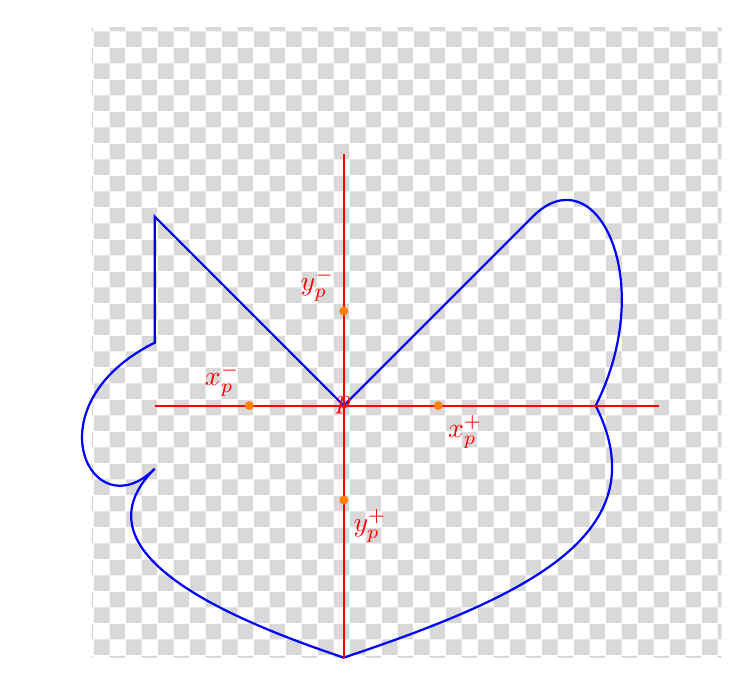
\begin{tikzpicture}[scale=0.8]

% Draw the grid pattern
\fill[pattern color=gray!30,pattern=checkerboard] (-4,-4) rectangle (6,6);

% Define the blue outline of the shape
\draw[blue, thick] 
    (-3,3) .. controls (-2,2) and (-1,1) .. (0,0)
            .. controls (1,1) and (2,2) .. (3,3)
            .. controls (4,4) and (5,2) .. (4,0)
            .. controls (5,-2) and (3,-3) .. (0,-4)
            .. controls (-3,-3) and (-4,-2) .. (-3,-1)
            .. controls (-4,-2) and (-5,0) .. (-3,1)
            -- cycle;

% Draw the red cross lines
\draw[red, thick] (-3,0) -- (5,0);
\draw[red, thick] (0,-4) -- (0,4);

% Mark the orange points
\fill[orange] (-1.5,0) circle (2pt);
\fill[orange] (1.5,0) circle (2pt);
\fill[orange] (0,1.5) circle (2pt);
\fill[orange] (0,-1.5) circle (2pt);

% Label the axes
\node[above left, red] at (-1.5,0) {$x_p^-$};
\node[below right, red] at (1.5,0) {$x_p^+$};
\node[above left, red] at (0,1.5) {$y_p^-$};
\node[below right, red] at (0,-1.5) {$y_p^+$};

% Label the center point
\node[red] at (0,0) {$p$};

% Add a small gap to separate the label from the cross
\node[red] at (0.1,0.1) {};

\end{tikzpicture}
\end{document}